\documentclass[12pt]{article}
\usepackage{textcomp}
\usepackage{url}
\usepackage{graphicx}
\usepackage{float}
\usepackage{booktabs}
\usepackage{enumitem}
\usepackage{listings}
\usepackage{emptypage}
\usepackage{subcaption}
\usepackage{multicol}
\renewcommand{\ttdefault}{jkptt}

\usepackage[T1]{fontenc}

\usepackage[usenames,dvipsnames]{xcolor}
\usepackage{amsmath, amsfonts, mathtools, amsthm, amssymb}
\usepackage{mathrsfs}
\usepackage{cancel}
\usepackage{bm}
\usepackage{setspace}


\usepackage{thmtools}
\usepackage[framemethod=TikZ]{mdframed}
\mdfsetup{skipabove=1em,skipbelow=0em}

\makeatletter

\declaretheoremstyle[headfont=\bfseries, bodyfont=\normalfont, mdframed={ nobreak, innerbottommargin=10pt, innertopmargin=7pt} ]{box}
\declaretheoremstyle[headfont=\bfseries, bodyfont=\normalfont, numbered=no, mdframed={ rightline=false, topline=false, bottomline=false}]{proof}

\declaretheorem[style=box, name=Definition]{definition}
\declaretheorem[style=proof, name=Proof]{_proof}
\renewenvironment{proof}[1][\proofname]{\begin{_proof}}{\end{_proof}}

% Figure support 
\usepackage{import}
\usepackage{xifthen}
\usepackage{pdfpages}

\newcommand{\incfig}[2][1]{%
    \def\svgwidth{#1\columnwidth}
    \import{./figures/}{#2.pdf_tex}
}

\graphicspath{
    {images/}
}




\begin{document}

\begin{center}
{\Large Representations and Representation Learning} \\
\vspace{5mm}
{\large Bryan Chiang and Jeanette Bohg}
\end{center}

\section*{Overview}

\subsection*{States and Representations}

Consider the following system consisting of a walking robot. The \textbf{state} is a quantity describing the key aspect of a system. In this example, the state may consist of information about the robot's 3D structure and motion. How do we actually parameterize the state? In this context, a \textbf{representation} refers to the literal data format used to describe the state, often dependent on the task at hand. Numerous representations are possible for a given state; for instance, we could choose to use any selection of joint angles, velocities, positions or the pose of the robot.

\begin{figure}[H]
  \caption{Walker robot from the DeepMind Control Suite.}
  \centering
  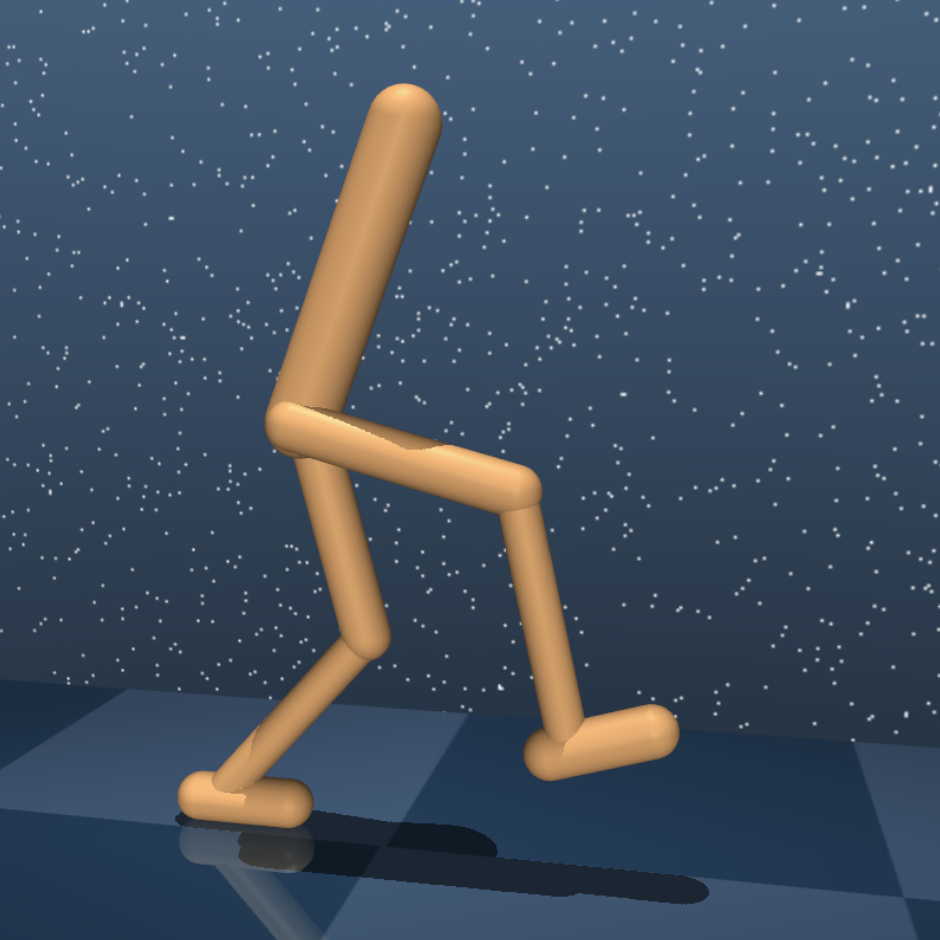
\includegraphics[width=4cm]{walker}
\end{figure}


In a \textbf{dynamical} system, the state is not static and evolves over time. Here, we would expect the robot to move. We denote the state at time $t$ as $x_{t}$. \textbf{Markov models} (specifically, Markov chains) are systems that possess the \textbf{Markov property}: future states only depend on the current state, not past states. In other words, state $x_{t+1}$ is conditionally independent of past states $x_{1}, x_{2}, \dots, x_{t-1}$ given current state $x_{t}$, and we can predict the state at the next timestamp given the current state according to specific dynamics of the system, or $f(x_{t}) = x_{t+1}$. For instance, if the state contains the current angular velocity of a joint, we can predict the joint angle at the next time step. $f(\cdot)$ may be a non-linear function, and we often assume that the dynamics are constant over time for simplicity. In the diagram below, the arrows indicating the chain of dependence.

\begin{figure}[H]
  \caption{Diagram of a Markov chain.}
  \centering
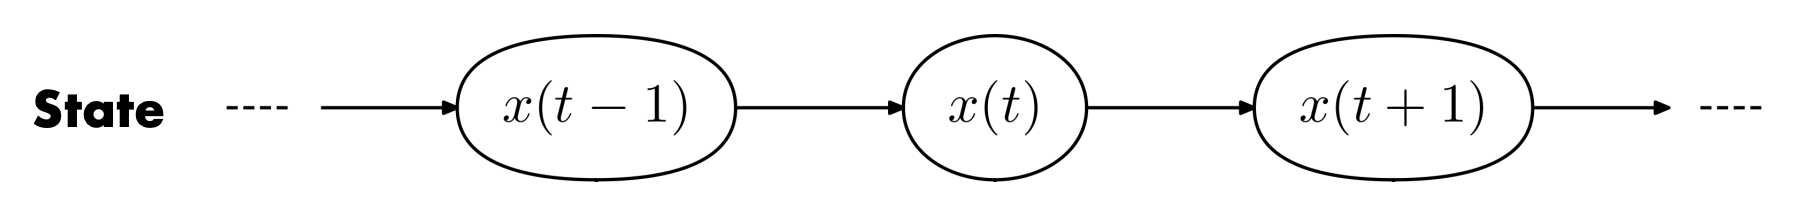
\includegraphics[width=12cm]{markov-model}
\end{figure}

In practice, the state at time $t$ is unknown. Our job is to use noisy observations to estimate the the true state: a process called \textbf{state estimation}. Such systems are termed \textbf{hidden Markov models} (or HMMs) since the state is "hidden". We assume that the states $x_{t}$ behave as a Markov process. We also assume that observation $z_{t}$ at time $t$ only depends on the state at that time, $x_{t}$. In other words, $f(x_{t}) = x_{t}$. The observation $z_{t}$ is conditionally independent of all previous states and observations given $x_{t}$. Hidden Markov models are partially-observable, while Markov chains are fully observable.

\begin{figure}[H]
  \caption{Diagram of a hidden Markov model.}
  \centering
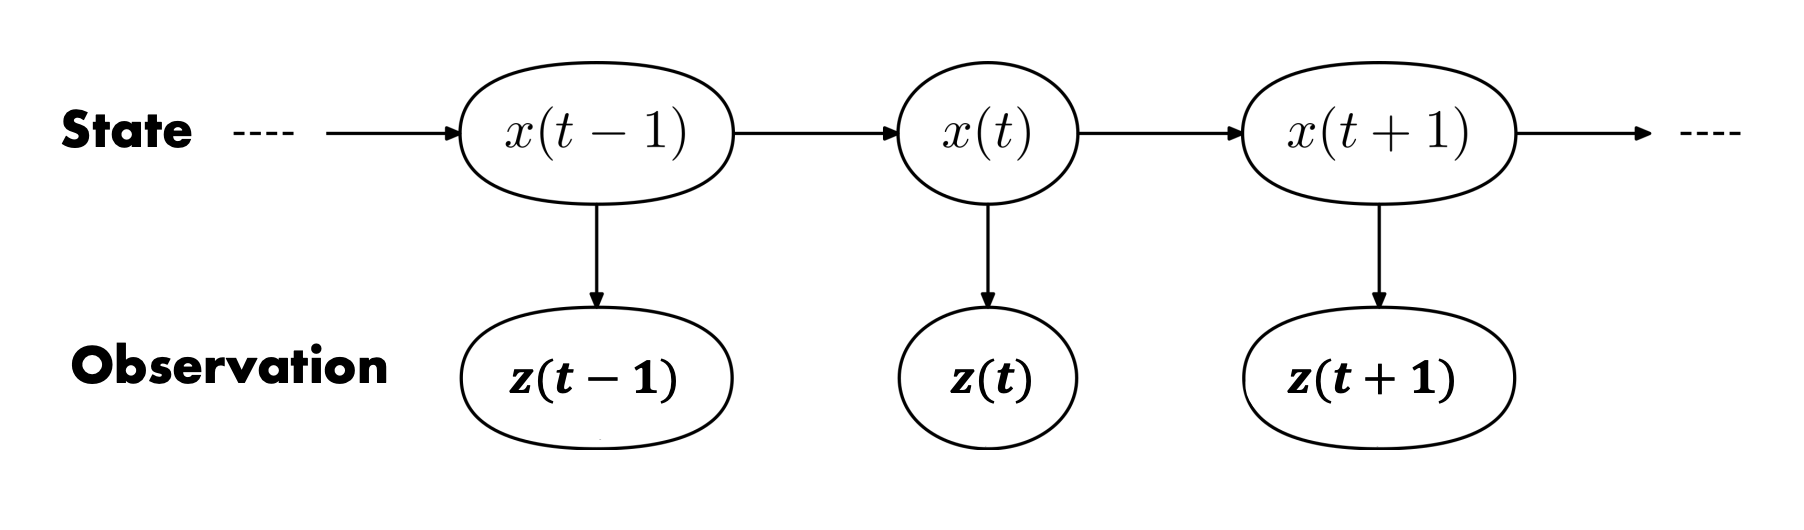
\includegraphics[width=12cm]{hmm}
\end{figure}

Let's make this concrete with a vision example. If we're a self-driving car with the following point-of-view, we'd be want to know the state of all the pedestrians to avoid any collisions: 3D locations, bounding boxes (size), possibly velocities of everyone. However, this information is not given to us and therefore must be estimated from our captured observations, which could be a pair of stereo images, RGB frames, or LIDAR data.

\begin{figure}[H]
  \caption{RGB image observation of pedestrians from a car POV.}
  \centering
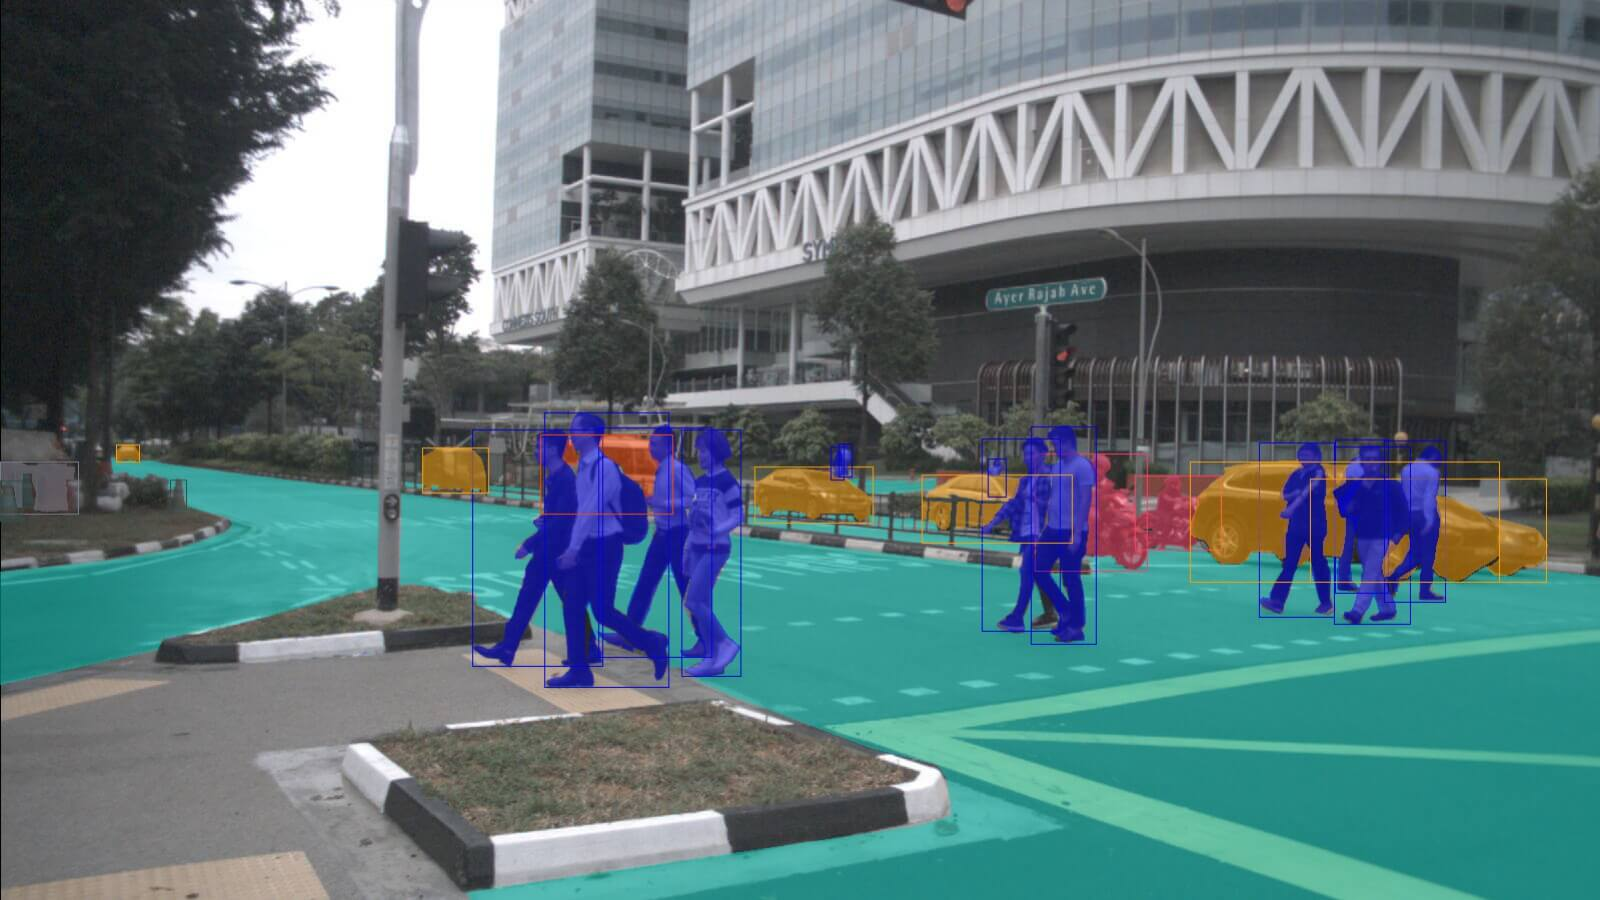
\includegraphics[width=10cm]{nuscenes}
\end{figure} 

In future lectures on optimal estimation, we will account for manually applied actions or control inputs in these Markov processes that affect the state. Specifically, instead of $f(x_{t}) = x_{t+1}$, we will have $f(x_{t}, u_{t}) = x_{t+1}$, where $u_{t}$ is the control input or action taken at time $t$ (such as rotating a joint motor to move the legs). Markov chains generalize to \textbf{Markov decision processes (MDPs)}, and hidden Markov models generalize to \textbf{partially observable Markov decision processes (POMPDPs)}.

\subsection*{Generative and Discriminative Approaches}

How can we estimate the state from observations? Let's consider the task of estimating an object's pose (state $x$) from an input RGB image (observation $z$). A 6D pose refers to both the objects 3D translation and 3D rotation (6 parameters total). 

\begin{figure}[H]
  \caption{PoseCNN (2018) network is an example of a discriminative model.}
  \centering
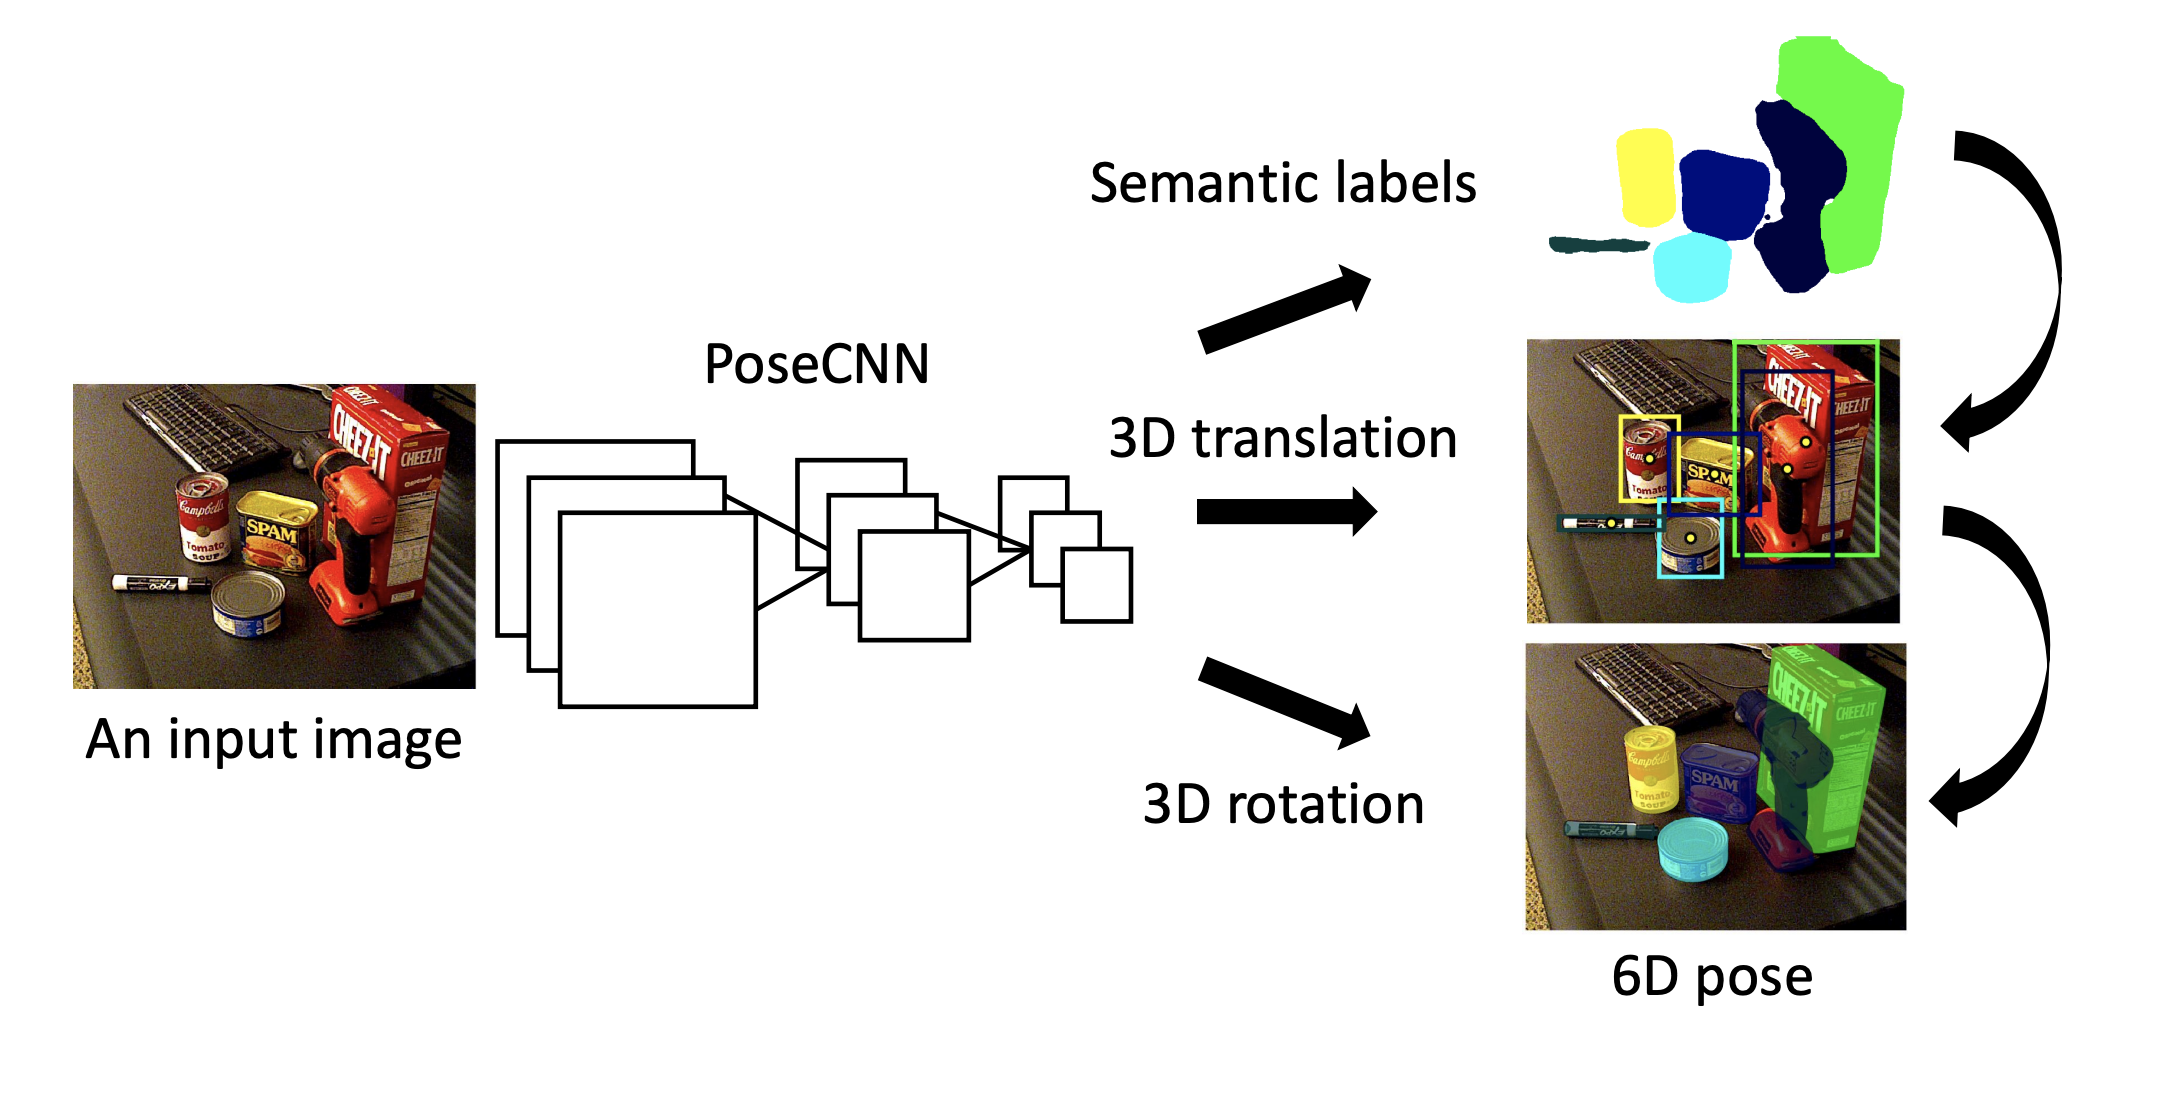
\includegraphics[width=12cm]{pose-cnn}
\end{figure}


We describe two approaches at a high-level; we will delve into specifics later in the course. First, a discriminative model aims to learn the parameters $\theta$ for a functional form of $p_{\theta}(x|z)$ from the observations. For instance, we could train a neural network to directly map the input image to the most likely output pose. Second, in contrast, a generative model aims to learn the parameters for functional forms of $p(z|x)$, $p(x)$ separately to model the joint $p(z, x)$ via Bayes Rule. For instance, we can sample a 3D pose prediction from $p(x)$ and measure $p(z|x)$ by comparing the differences between the image coordinates of the predicted 3D poses's 2D projection on the image plane with the actual observed image coordinates. To learn more about the differences about discriminative and generative models, please refer to the CS229 notes.

\section*{Representation Learning}

\subsection*{Representations in Computer Vision}

We turn our attention to representations in computer vision, which can have multiple meanings depending on the context. 

\begin{figure}[H]
  \caption{Input, intermediate, and output representations.}
  \centering
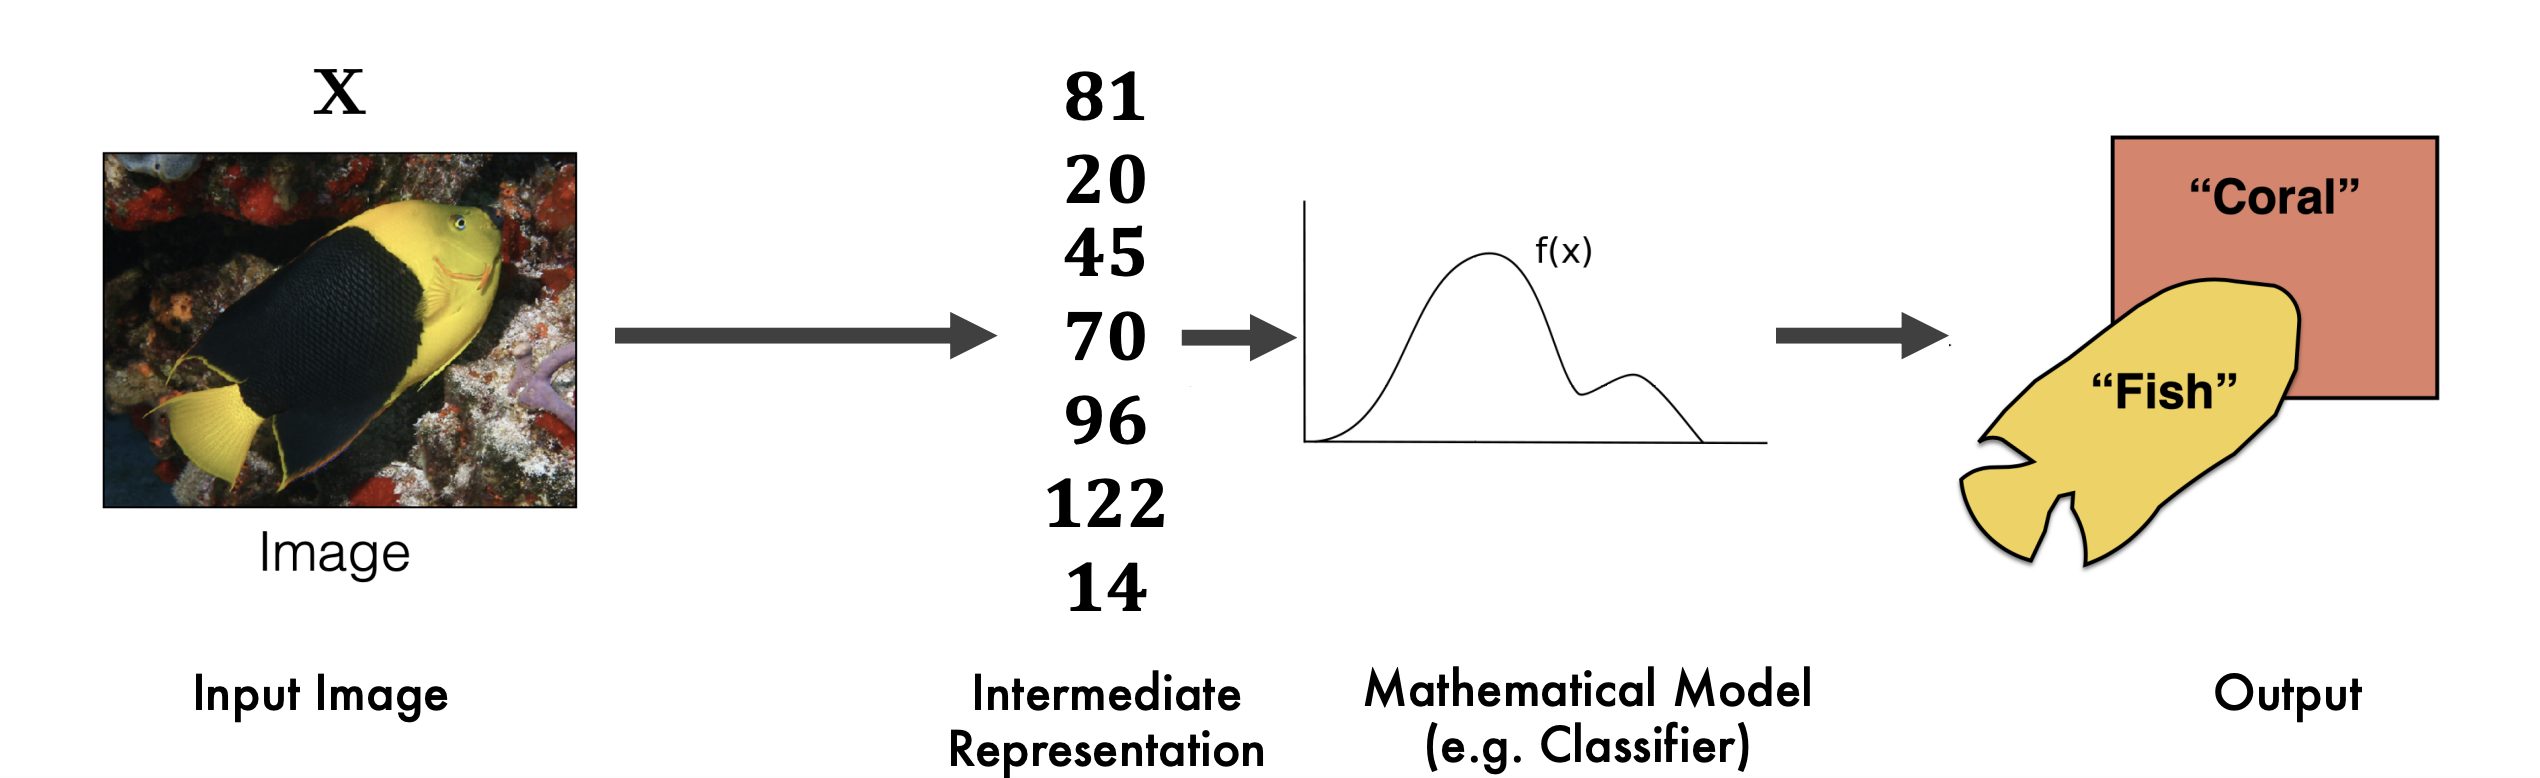
\includegraphics[width=14cm]{cv-reps}
\end{figure}

On one end of the spectrum, when we talk about \textbf{input representations}, we are referring to the raw sensor data format that was used to capture the input. In the above example, our input is the 3D scene within the ocean containing the fish. Depending on sensor choice, the input representation of the scene could be images, depth frames, point clouds, or any other imaging modality. Even within a specific form, there are subtle differences in the input representation. For instance, color vs. grayscale, stereo vs. monocular, RGB vs. HSV (image color spaces). On the other end of the spectrum, \textbf{output representations} succinctly describe the high-level key aspects of the scene that are necessary for decision-making and completing downstream tasks. If we were a biologist and our goal was to count the number of fish we encounter, the relevant output representation may be the "Fish" label on the output side, or even a more specific label indicating the species of the fish. However, if we (the camera) were a drone attempting to navigate the coral reef, we may be more interested in estimating the 6D pose and 3D bounding box of the fish, which would be useful to incorporate into our trajectory planning. In between input and output representations lie \textbf{intermediate representations}, which are compressed, low-dimensional vector representations that summarize the high-dimension sensory data (input). Intermediate representations are derived from the input representation, and subsequently, output representations are derived from the intermediate representations. 

Some natural questions at this point are:

\begin{enumerate}[]
  \item Since representations are so key for decision-making, what makes for a good representation? 
  \item How do we actually obtain intermediate and output representations?
\end{enumerate}

\subsection*{Representation Criteria}

Bengio proposed several...

\subsection*{Traditional CV and Interpretable Representations} 

The traditional ($\approx$ pre-2012) computer vision pipeline is as follows.

\begin{figure}[H]
  \caption{Classical CV pipeline for extracting representations. Intermediate representations can be used to derive higher-level intermediate representations. }
  \centering
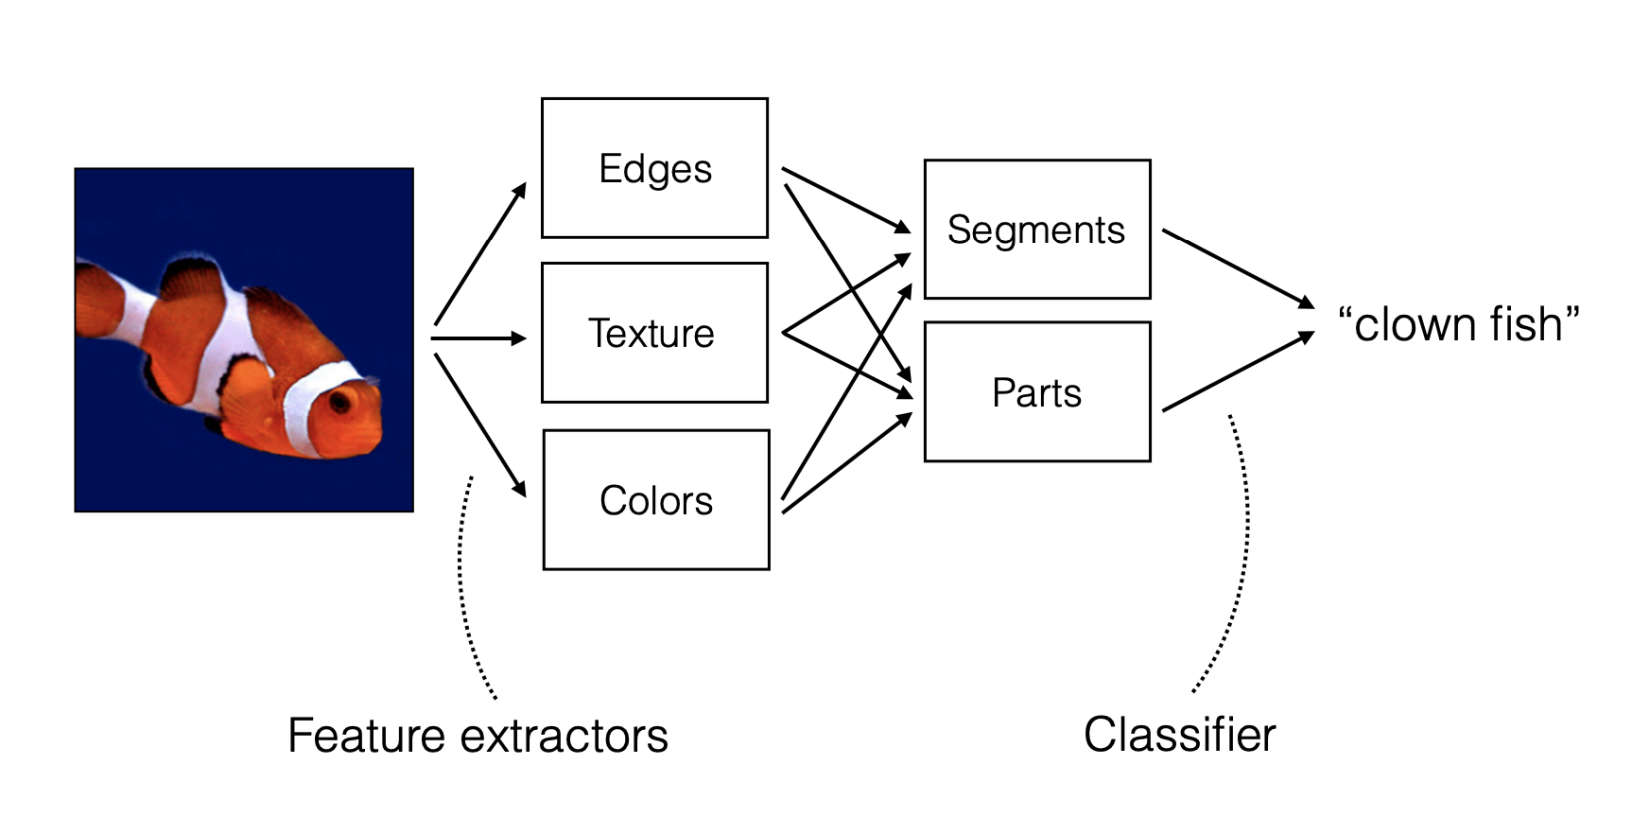
\includegraphics[width=14cm]{trad-cv}
\end{figure}

Here, our intermediate representations are combinations of hand-crafted features extracted from the image input representation. The specific choices of features (descriptors) is flexible. For instance, if we believe that specific stripes or designs on a fish's body may be distinguish it from other types of fish or things in the sea, then we could exploit those specific patterns by extracting edges and colors as our intermediate representation. To extract the output representation (here a class label), our intermediate representation is fed into classifier, which incorporates the intermediate representations to make a decision either in a learned manner or based on more manually-defined heuristics. As a simple example, I can define a heuristic that if the histogram of colors in the image contains a high amount of oranges and whites, we may say that the image is likely to contain a clownfish. Much classical literature has focused on developing new feature extractors, often based on image processing and filtering methods. While specific methods are out of this class's scope, we provide several references for further reading at the end of this document. The primary benefit of classical feature extraction methods is that they result in \textbf{interpretable representations}: because we designed these methods by hand, we can easily explain why specific output representations were chosen. This can be especially important for downstream tasks with high stakes, perhaps in legal or medical domains. However, the downside is that coming up with these feature extractors is a tedious process, requiring significant amounts of time and domain expertise that may not be available.

\subsection*{Modern CV and Learned Representations}
Modern computer vision methods ($\approx$ 2012-present) replace manually extracted features \textbf{learned representations}. Through an iterative learning process, we let the layers of parameters of a (convolutional) neural network learn by themselves how to determine intermediate representations that will lead to extracting the most accurate output representations.

\begin{figure}[H]
  \caption{Learned intermediate representations. We do not choose specific feature components to use, hence the blank boxes.}
  \centering
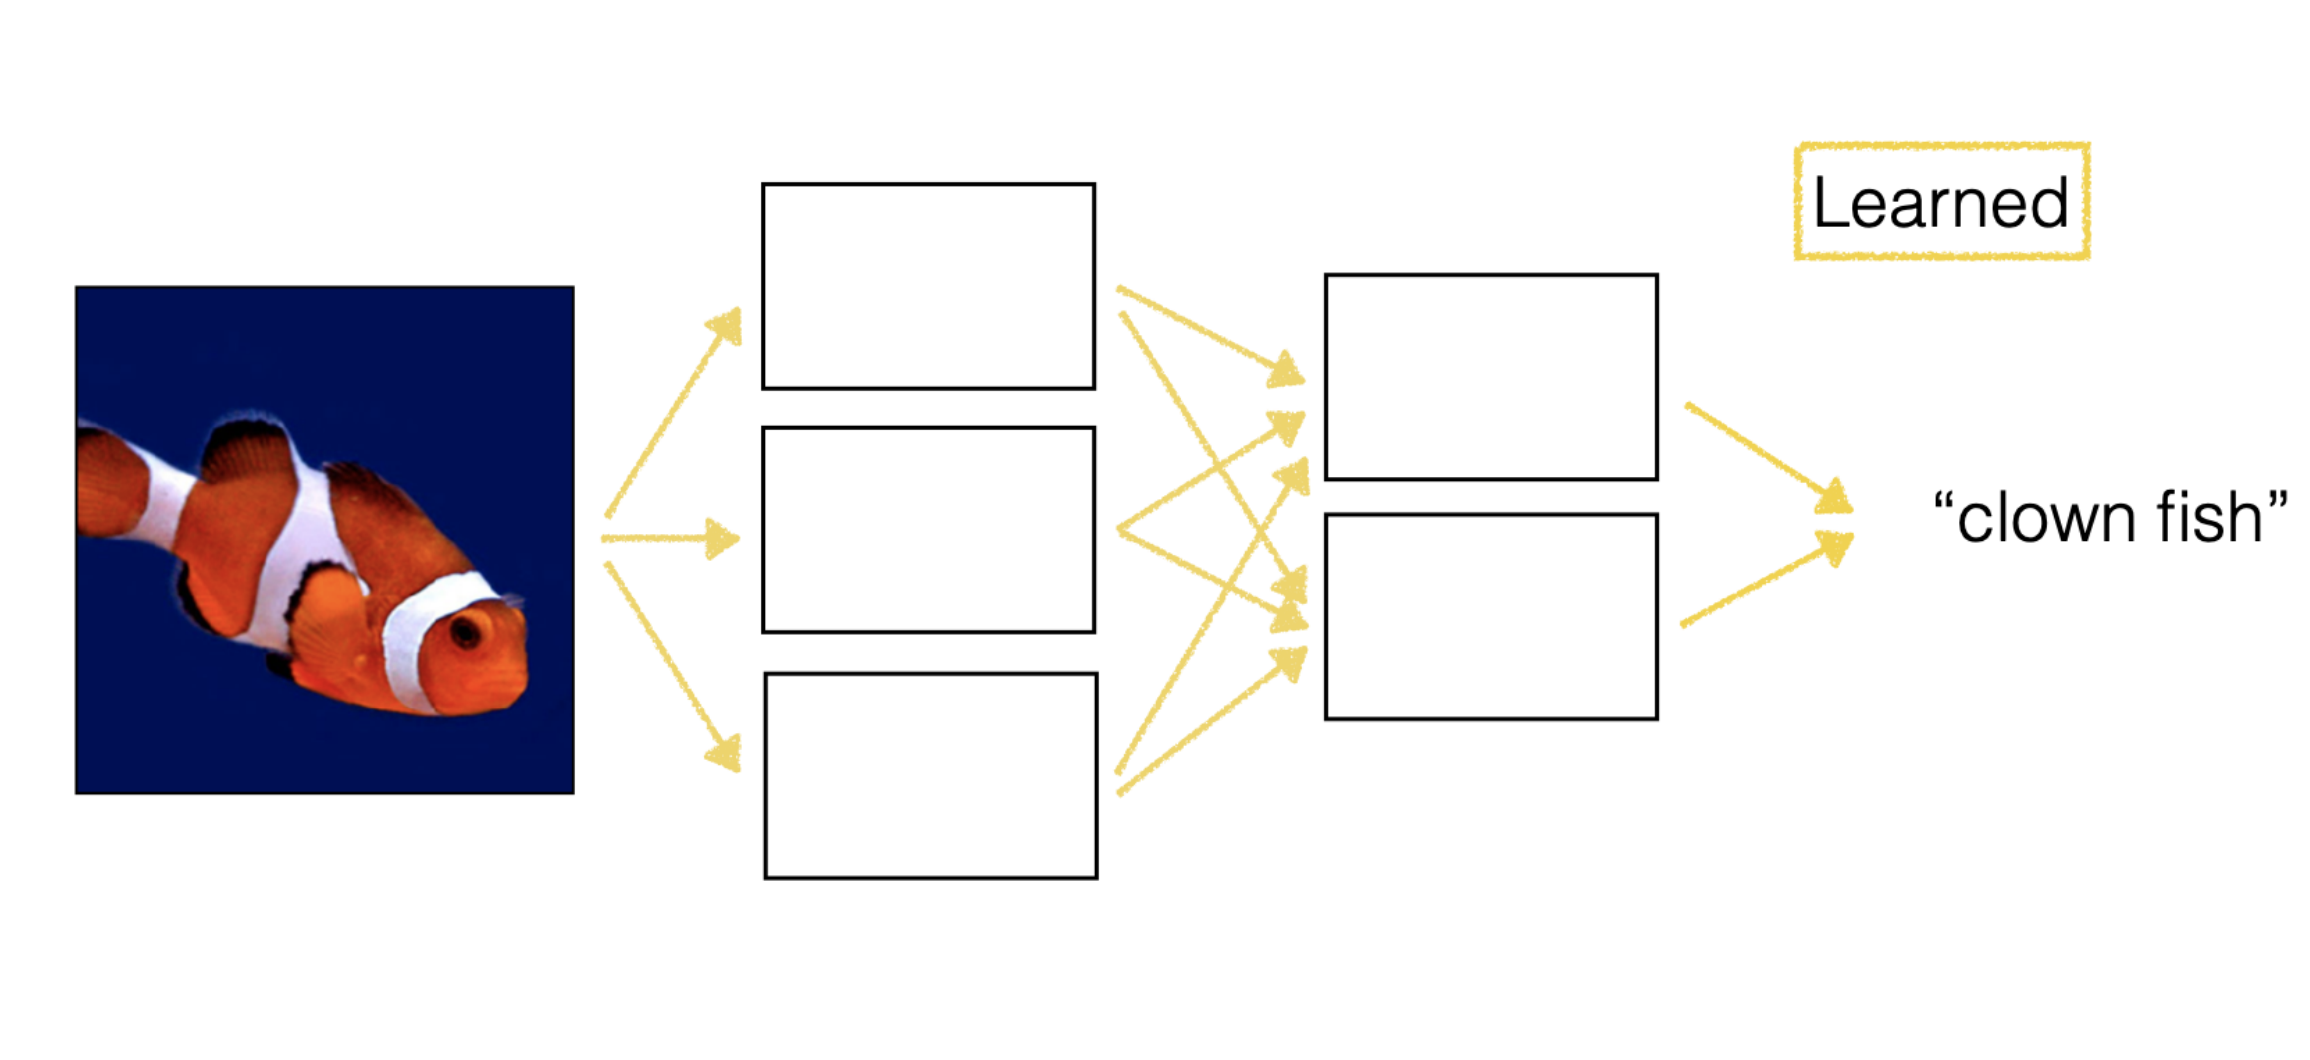
\includegraphics[width=14cm]{learned-cv}
\end{figure}

While learned representations can extract output representations accurately and robustly, the downside is that they lack the interpretability of classical representations. Several methods for interpreting learned representations to understand why they perform so well and how to improve them. Zeiler and Fergus (2014) analyzed the specific image patches that activate filters the most strongly for each layer in a CNN trained on ImageNet. What they discovered was that the learned representations resembled the traditional extracted features (such as edges, textures, body parts). In other words, the pipeline was capable of learning its heuristics that were just as advanced as what a human could come up with.

\begin{figure}[H]
  \caption{Different levels of learned intermediate representations represent those of a traditional pipeline.}
  \centering
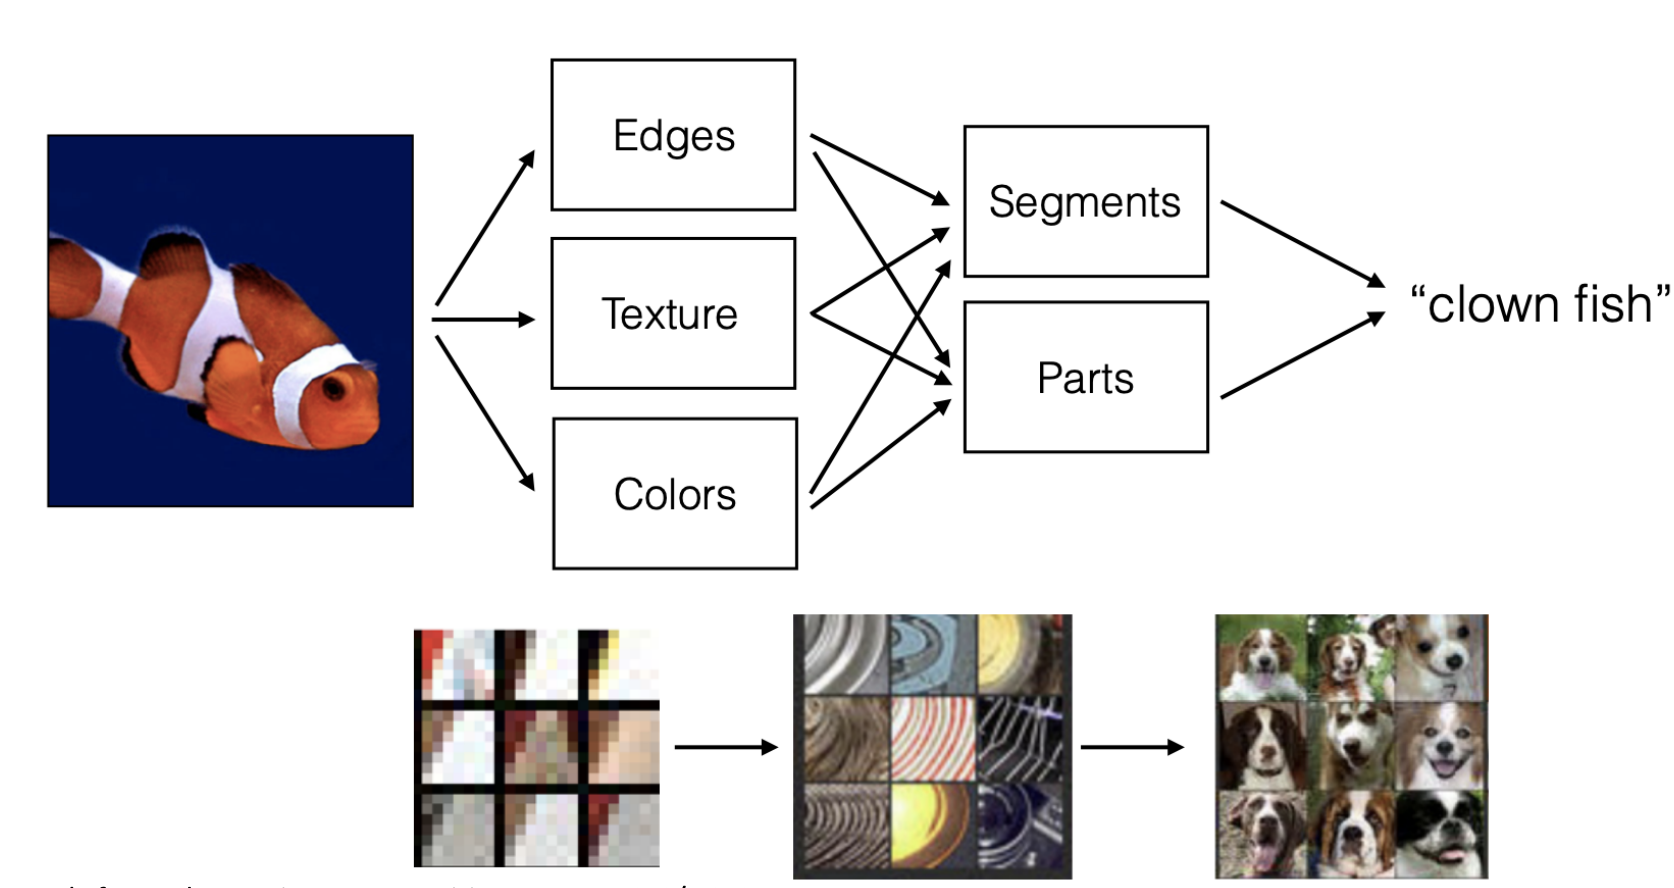
\includegraphics[width=14cm]{interpreting}
\end{figure}

Another approach to understanding intermediate representations is projecting them to a lower dimensional space so that we can plot and interpret them. One popular technique for achieving this is tSNE (Van der Maaten and Hinton, 2008), which performs dimensionality reduction on high-dimensional intermediate representations by minimizing the KL-divergence of joint probabilities (based on data similarity) between the low-dimensional embeddings and original high-dimensional representations. We expect that images from the same class will be geographically clustered near each other; we can use tSNE to sanity check that our neural network indeed learns that images with the same label are also similar visually.
 
\begin{figure}[H]
  \caption{Visualization of tSNE embeddings on the MNIST dataset.}
  \centering
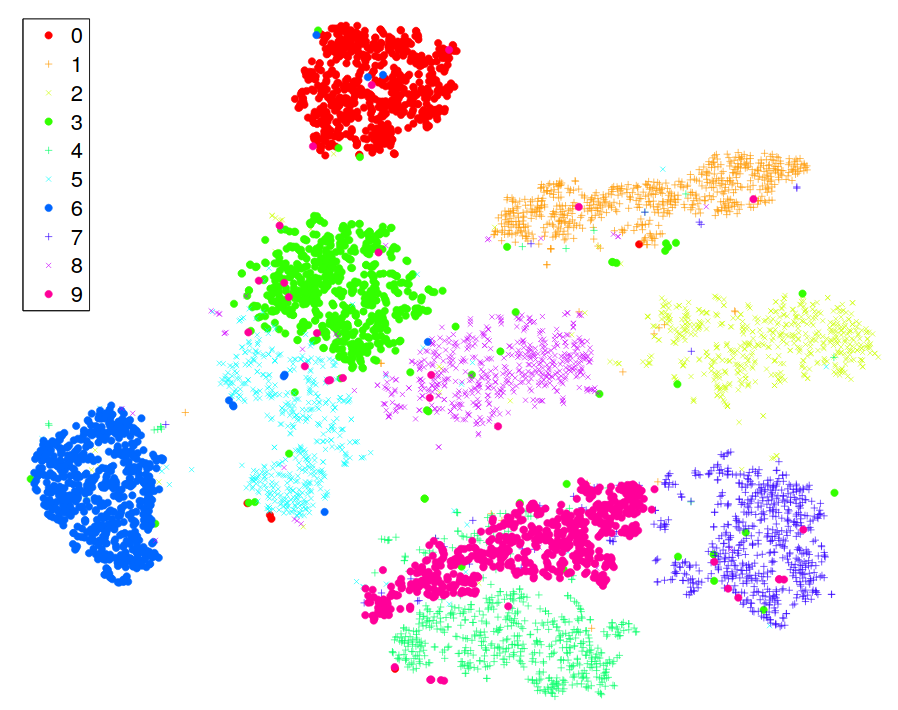
\includegraphics[width=8cm]{tsne}
\end{figure}

\subsection*{Unsupervised and Self-Supervised Learning}

In a traditional supervised learning formulation, we can teach our model (probably a CNN) to learn given a loss function and a dataset of $(x_{i}, y_{i})$, where $x_{i}$ is the input representation (data) and $y_{i}$ is the output representation (label). In practice, data is abundant. However, labels are expensive to acquired and can require specialized knowledge. Can we learn meaningful representations from data \textit{without} labels? Consider the \textbf{autoencoder} architecture shown below. The goal of an autoencoder is to learn to perfectly reconstruct the input image. This is represented by the reconstruction loss, which is defined as the difference between the output representation, $\mathcal{F}(\mathbf{X})$, and the input image, $ \mathbf{X}$. We expect that the output representation should be identical to the input representation. The intermediate representation $ \mathbf{z}$, the compressed image code in the latent space located at the middle of the network. Intuitively, we expect that if the second half of the network $\mathcal{F}$ is able to reconstruct the input from  $ \mathbf{z}$, then $ \mathbf{z}$ is a useful and informative compressed version of the input representation. For this reason, we say that $ \mathbf{z}$ is the output of the \textbf{bottleneck layer}.

\begin{figure}[H]
  \caption{Autoencoder architecture for unsupervised learning. $\mathcal{F}$ is the autoenconder, $ \mathbf{X}$ is the input image, $\mathbf{\hat{X}}$ is the reconstructed input image.}
  \centering
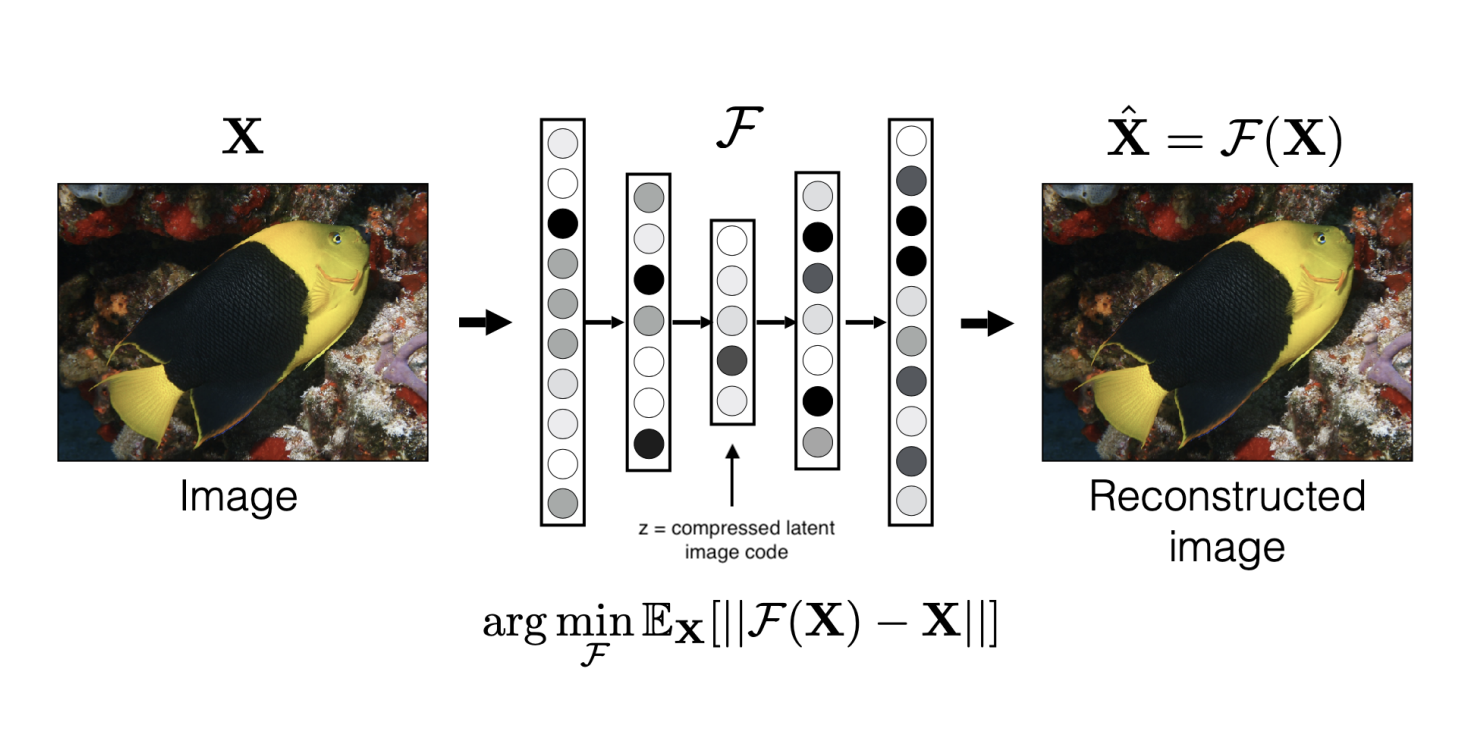
\includegraphics[width=14cm]{ae}
\end{figure}

We say that an autoencoder performs \textbf{unsupervised learning} since it requires no external labels aside from the input image (which may be viewed as the label itself). In a similar vein, \textbf{self-supervised learning} masks out part of the input to use as the output label. For instance, we can keep all pixels below the image diagonal as the input, and all the pixels above the diagonal as the output. Given the lower portion, the task would be to reconstruct the upper portion of the image. The hope is that the network would still learn meaningful representations about the input images to achieve this task. This has been empirically shown to some extent in the following manner. Given an autoencoder trained on a large amount of unlabeled data, we can obtain the compressed intermediate representation $ \mathbf{z}$ with the first half of the network (also called the \textbf{encoder}). Then, with only a small amount of labeled data, we can train a classifier on top of the intermediate representation $ \mathbf{z}$ to accurately predict the output representation since the autoencoder has already done the heavy lifting of learning a meaningful representation for the input.

\end{document}
